\documentclass[journal]{IEEEtai}

\usepackage[T1]{fontenc}
\usepackage[utf8]{inputenc}
\usepackage{cite}

\usepackage[colorlinks,urlcolor=blue,linkcolor=blue,citecolor=blue]{hyperref}

\usepackage{color,array}

\usepackage{graphicx}

\usepackage{graphicx}

\newtheorem{theorem}{Theorem}
\newtheorem{lemma}{Lemma}
\setcounter{page}{1}


\begin{document}


\title{ Learning the unlearnable: Generating Hungarian text using transformers } 


\author{György J. Author, György K. Author, and Márió Z. Author
\thanks{This work was made as a final assignment for the subject ``Deep Learning in Practice with Python and LUA'' (course ID: BMEVITMAV45) supervised by Budapest University of Technology and Economics Faculty of Electrical Engineering and Informatics, 1117 Budapest, Magyar tudósok körútja 2. }
\thanks{Gy. J. Author is a student of Budapest University of Technology and Economics Faculty of Electrical Engineering and Informatics, 1117 Budapest, Magyar tudósok körútja 2. (e-mail: jozsagyorgy@edu.bme.hu).}
\thanks{Gy. K. Author is a student of Budapest University of Technology and Economics Faculty of Electrical Engineering and Informatics, 1117 Budapest, Magyar tudósok körútja 2. (e-mail: kurucz.gyorgy@edu.bme.hu).}
\thanks{M. Z. Author is a student of Budapest University of Technology and Economics Faculty of Electrical Engineering and Informatics, 1117 Budapest, Magyar tudósok körútja 2. (e-mail: zellermario@edu.bme.hu).}}

\markboth{Deep Learning in Practice with Python and LUA final assignment, Vol. 01, No. 1, December 2020}
{First A. Author \MakeLowercase{\textit{et al.}}: Bare Demo of IEEEtai.cls for IEEE Journals of IEEE Transactions on Artificial Intelligence}

\maketitle

\begin{abstract}
The prevalence of Natural Language Processing has grown drastically in the last decades. Today, NLP is used in a wide variety of applications. Companies use so-called chatbots for costumer interactions, capable of understanding and answering costumers' questions. Speech recognition software solutions help the disabled in online interactions, and contribute to the average user's user experience. Other applications include the translation, summarization, and extraction of text, and the detection of intent or urgency of texts. Generating syntactically sound text is a difficult exercise that has been studied in great length. Recently, developments in this field has allowed the creation of software capable of generating texts that pass the Turing-test in the form of GPT-3. However, most text generating agents are focused on the English language, while other, more complex languages have received less attention. In this assignment, we create a model for generating Hungarian news articles.
\end{abstract}

\begin{IEEEImpStatement}
Chatbots are a popular technology in online interaction. They reduce the load on human support teams and offer continuous 24-7 support to customers. Likewise, the recent popularity of GPT-3 and BERT language models shows the need for high-functioning Natural Language Processing solutions. However, most of these efforts are centered around the English language. The language model we introduce in this paper offer an alternative to these English models, as it is working with the much more complex Hungarian language, by generating news articles, based on popular Hungarian news outlets.
\end{IEEEImpStatement}

\begin{IEEEkeywords}
Enter key words or phrases in alphabetical order, separated by commas. For a list of suggested keywords, send a blank e-mail to \href{mailto:keywords@ieee.org}{\underline{keywords@ieee.org}} or visit \href{http://www.ieee.org/organizations/pubs/ani_prod/keywrd98.txt}{\underline{http://www.ieee.org/organizations/pubs/ani\_prod/keywrd98.txt}}
\end{IEEEkeywords}



\section{Introduction}

\IEEEPARstart{T}{he} demand for good computer language agents is ever growing. Natural Language Processing (NLP) offers a solution to this with deep neural networks designed to learn the syntactic and semantic structure of natural language. Recent development of the transformer architecture\cite{vaswani2017attention} has helped models reach a level of sophistication previously unseen in Recurrent Neural Network (RNN) based text generators. Solutions such as GPT-3\cite{brown2020language} (Generative Pre-trained Transformer 3) and BERT\cite{devlin2019bert} (Bidirectional Encoder Representations from Transformers) offer high quality generated text capable of passing the so-called Turing-test\cite{TuringMind}.

However, most implementations focus on English language processing, whereas text generators in other languages are sparse and lack the high level of sophistication in language understanding and syntactic correctness. 

Furthermore, non-English languages pose additional challenges as linguistic properties differ from language to language. Particularly, agglutinative languages challenge these models, as words have a range of different suffixes, making it more difficult for a language learning model to learn a semantic understanding of input text.

\section{Objective}
Our goal in this assignment was to create an NLP model capable of generating texts mimicking  the styles' of popular Hungarian news articles from outlets such as {\it index.hu} and {\it origo.hu}. Upon supplying the model a sentence or a beginning of a sentence as a prompt, we expect it to generate an output of a whole news article

\section{Challenges}
Previous works have been focusing parts and aspects of the Hungarian language, such as identification of zero copulas\cite{Dmtr2020MuchAA}, and understanding legal texts in Hungarian\cite{gorog2019legal}, however, few have attempted to generate lifelike Hungarian text. The language itself has a reputation of being particularly difficult to learn for foreigners. This is because its agglutinative nature and difficult syntactic rules. Hungarian has been called the most creative language in the world, as you can play with the order and the cases, and moreover, with the suffixes and prefixes, too. These complex syntactic rules make Hungarian a very difficult language to master even for humans, and certainly for neural networks such as our model.

Furthermore, language processing models, such as BERT and GPT-2 require an immense amount of time and computer resources to learn the complex relations of language. Even GPT-2, the predecessor of GPT-3 struggled to generate lifelike texts, and understand human input, even though it was created with millions of dollars worth of technology and dozens of state-of-the-art experts in the field. We can not afford millions of dollars' worth of computer resources, having to use free alternatives, such as Google collab.


\section{Methodology}
For implementing the text generating agent, we needed to solve multiple problems. The first challenge presented itself as databases of cleaned Hungarian texts don't exist. We needed to scrape it for ourselves. After collecting the data, we needed to design a model to generate the output text, given an initial prompt. Finally, we needed to train the network with the collected data, so that the model can learn the Hungarian language.  

\subsection{Collecting the data}
Our initial plan was to use the database on \href{https://mek.oszk.hu/}{https://mek.oszk.hu/}, containing tens of thousands of Hungarian documents. However, the lack of easily usable API or centralized index-registry would have made it difficult to collect enough data for the training phase, leading to us ultimately deciding against this source.

Our attention turned to popular Hungarian news sites, particularly \href{https://index.hu/}{https://index.hu/} and \href{https://www.origo.hu}{https://www.origo.hu}. These particular sites were ideal as they provided regular HTML paths and centralized pages containing all previous articles. 

We first scraped all the links of articles written in the past 4 years from both outlets. Then, we proceeded to download the HTML body of all links gathered. This would have resulted in more than 300,000 Origo articles and a similar amount of Index articles. However, due to time constraints, we stopped the process prematurely, only gathering articles in the tens of thousands. Precisely, we used 15991 articles from Origo and 62184 articles from Index.

We separated the Origo and Index articles from each other, as they have vastly different styles. This separation meant that we could train our model later on to generate articles of different styles. 

The data was reformatted, so that one article was exactly one line in the text file. This was to easily separate articles from each other.

The data sets were then shuffled, as to mix them in time. This prevented a bias in training where the training, validation and test data sets would result in being disjunctive in time. This resulted in data being representative of the general style of the outlet, and not the time period. 

\subsection{designing the model}
The design of the model was an important decision. Since Hungarian text generating pre-trained frameworks do not exist, we were forced to build the model from the ground up. We have considered two architectures for the project. 

The first option was a Recurrent Neural Network (RNN) with Long-Term Short Memory\cite{lstm} (LSTM) cells. These networks are capable of generating text tokens based on the previously generated tokens, which contribute to the model's ability to make semantic connections in long-term syntactic structures.

The second option was a Transformer\cite{vaswani2017attention} architecture. Transformers have recently been conceptualized, and have subsequently changed the landscape of Natural Language Processing. With the utilization of self-attention layers, transformer models are capable of establishing long-term connections between text tokens, even to the point of generating new tokens based on the entire previous generated output. The attention layers are built for parallel processing of data, speeding up the training process by utilizing GPU cores. The major downside of this approach is because of the architecture's novelty, no standard implementation exists, forcing us to implement the whole architecture ourselves. This results in the implementation being sub-optimal.

We eventually decided to use a transformer-based network. The implementation is based on the original paper\cite{vaswani2017attention} describing the architecture. We used positional encoding according to the paper, and the decoder uses multi-headed attention layers that are activated by Dropout\cite{overfitting} layers and normalized via Layer Normalization\cite{ba2016layer}. The transformer itself is modified from the original design, the biggest difference is the omission of the input embedding, as the output is generated as the continuation of the prompt.

\subsection{Hyperparameter optimization}
For optimizing the hyperparameters, we used the Keras Tuner library. The results of these tunings can be seen on Fig. \ref{fig:hp}. 

In these graphs, ``dff'' denotes the size of the fully connected feed-forward network. ``num\_layers'' refers to the number of decoder layers. ``num\_heads'' is the number of attention heads and finally, ``d\_model\_per\_heads'' denotes the size of the input embedding divided by the number of attention heads.
\begin{figure*}
	\centering
  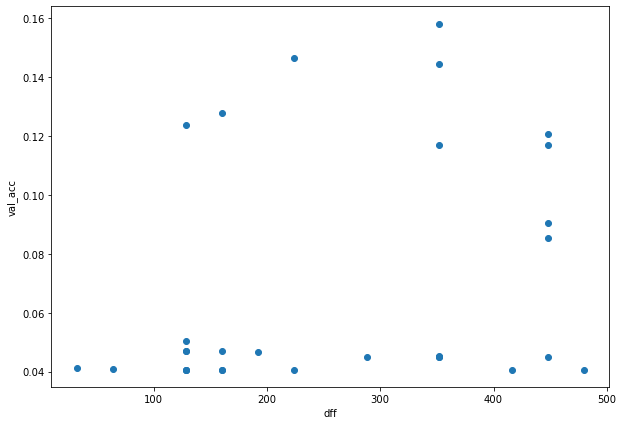
\includegraphics[width=0.45\linewidth]{fig/hp_dff.png}
  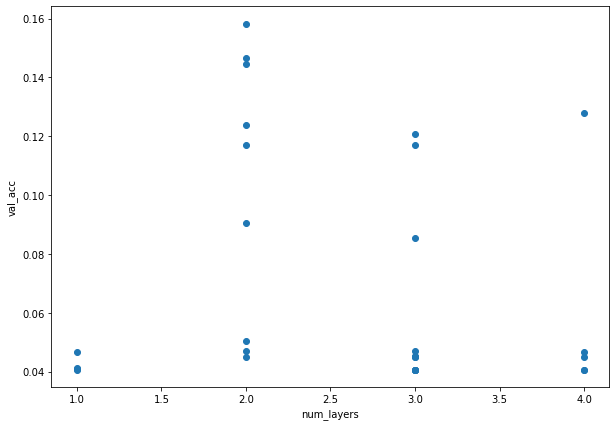
\includegraphics[width=0.45\linewidth]{fig/hp_num_layers.png}
  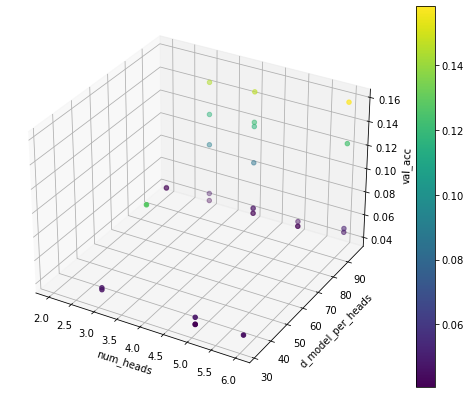
\includegraphics[width=0.5\linewidth]{fig/hp_num_heads_d_model.png}
  \caption{Accuracy as a function of the different hyperparameters.}
  \label{fig:hp}
\end{figure*}

\begin{figure*}
\centering
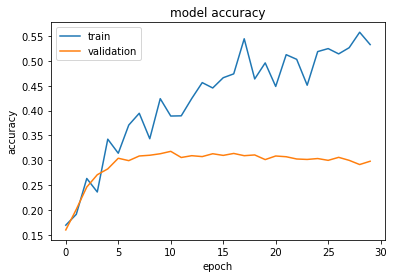
\includegraphics[width=0.45\linewidth]{fig/training_accuracy_30_epoch.png}
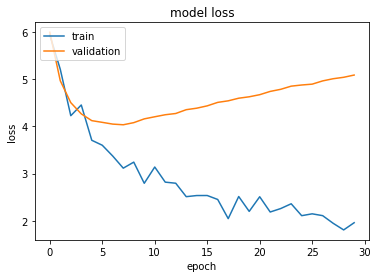
\includegraphics[width=0.45\linewidth]{fig/training_loss_30_epoch.png}
\caption{Accuracy and loss for the Origo model.}
\label{fig:training_origo}
\end{figure*}

\begin{figure*}
\centering
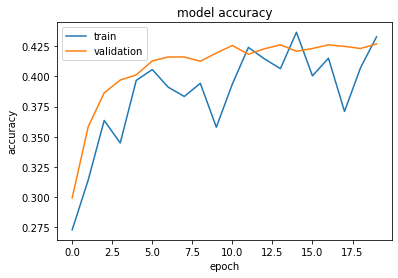
\includegraphics[width=0.45\linewidth]{fig/training_accuracy_index.png}
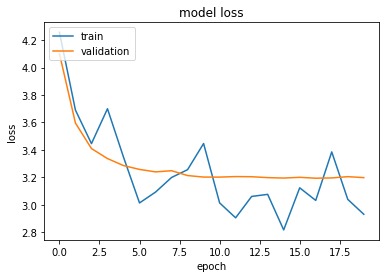
\includegraphics[width=0.45\linewidth]{fig/training_loss_index.png}
\caption{Accuracy and loss for the Index model.}
\label{fig:training_index}
\end{figure*}

\def\myrow#1#2{#1 & {\tt #2} \\}
\begin{table*}
\centering
\begin{tabular}{lp{12cm}}
\myrow{epoch 0}{sággalink Menőköették ütemredManink káPénink őköidejékáink átalakíttesztelésbűncselekmény őköőköidejérediszlőköütemrnyőZoltán őköőköőköZoltán}
\myrow{epoch 1}{A férfi a magyar év év és az első magyar labdarúgó. Egy magyar férfi a férfi az egyik férfi és egy férfi az egyik férfi a magyar válogatott és egy férfi}
\myrow{epoch 2}{A magyar női labdarúgó. A címvédő válogatott csatára hazai válogatott szövetségi kapitánya. A magyar csapatnak az Európa, a magyar válogatott szövetségi kapitányságra, a magyar}
\myrow{epoch 4}{Több százmillió forintot ért a Nemzeti Adó- és Vámos Alapítvány, az M0-as autóút forgalmú kilométerszetvédelem közelében}
\myrow{epoch 8}{Az elmúlt időszakban az Európai Uniónak a kilép az euróövezet kilépő kilépnek feltétellel. A tagországok. A kilé}
\myrow{epoch 16}{Az elmúlt tíz évben fokozatos egyre több biztonsági intézkedést jelentenek a veszélyhelyzetben, és a veszélyhelyzet megszűnteti, hogy a veszélyhelyzet idején további segítség}
\myrow{epoch 29}{A spanyol labdarúgóliga csoportkörében, az Atléticoa Barcelona edzője, a címvédő Real Madridban címvédő Real Solarisnak az argentin, Neymarnak a}
\end{tabular}
\caption{Text generated for an empty prompt during the training of the Origo model.}
\label{tab:training_origo}
\end{table*}

\section{Results}
After training our model of both data sets, we collected the results. The data shows that the model was able to learn Hungarian syntax as the training went on, as seen in Table \ref{tab:training_origo}. 

An interesting observation can be made from Figures \ref{fig:training_origo} and \ref{fig:training_index}, as the validation loss started to increase in the Origo data set at around epoch 6. This, coupled with e fact that the training loss continued to decrease is a clear sign that the model started overfitting for the training data set. This does not happen on the Index data set, leading to us postulating that this is a result of the difference in size in those sets (for reference: the Origo data set contained 15991 articles, while the Index set contained 62184, a factor of 3.89). This result is also supported by the accuracy divergence in the Origo data set, a phenomenon not seen in the Index data set.

To test the semantic learning of our model, we created a list of famous Hungarian politicians and parties, and fed the lists to the model one by one. To avoid very long articles, we maximized the generated text to at most 32 tokens. The result of these are contained in Tables \ref{fig:prompt_index} and \ref{fig:prompt_origo} We hypothesized that if the semantic understanding of the model was high, the generated articles would be highly different. Upon examining these generated texts, we found that the results were indeed different in tones and word usage, indicating our model's ability to pick up on semantic information and mannerisms.

\subsection{Test prompts}
For a list of interesting prompts, we sampled names and political parties from the following articles:
\url{https://magyarnemzet.hu/archivum/belfold-archivum/iranytu-intezet-ader-janos-helyet-varga-mihaly-foglalta-el-3885618/} \\
\url{https://index.hu/belfold/2017/02/27/botka_nepszerubb_orban_viktornal/} \\
\url{https://444.hu/2020/01/25/zavecz-csokken-a-fidesz-tabora-de-ettol-nem-lett-erosebb-az-ellenzek} \\

\def\myrowb#1#2{#1 & {\tt #2} \\}
\begin{table*}
\centering
\begin{tabular}{lp{14cm}}
\myrowb{Áder János}
{Áder János köztársaság és az Országgyűlésben  a közterület köztéri vendéglátósai és vendéglátósai , valamint a vendég közt}
\myrowb{Varga Mihály}
{Varga Mihály az első olyan magyar futballválogatott volt, ami nem a legjobb magyar válogatott futballistája. A magyar válogatott a világbajnokságon ezüstérmes volt az Európa-bajnokságo}
\myrowb{Tarlós István}
{Tarlós István főpolgármesterrel a főpolgármesterrel és az ellenzéki jelölttel is találkozik Karácsony Gergely főpolgármester-jelöltje, Karácsony szerint Karácsony Gergely és Tarlós István főpolgármester-jelölt, Karácsony }
\myrowb{Orbán Viktor}
{Orbán Viktor miniszterelnök a Facebook oldalára  posztolja, hogy az elmúlt két hónaphoz képest nem látszik, hogy a Fidesz miért indított kampányt, illetve az általa }
\myrowb{Navracsics Tibor}
{Navracsics Tibor egy éve került az Európai Unió luxembourgi programjába (EPP). A szervezet szerint egy luxembourgi székhely is szerepet vállalt az Európai }
\myrowb{Karácsony Gergely}
{Karácsony Gergely főpolgármester és a fővárosi Fidesz fővárosi frakcióülése összehozta azokat az ígéreteket, amelyeket az LMP szerint a következő hetekben kellene kilépnie a kormányt }
\myrowb{Hadházy Ákos}
{Hadházy Ákos független parlamenti képviselő, a képviselő a parlamentnek is elfogadta a parlamentet. A politikus szerint a képviselők nem szavaznak az LMP javaslatára: a parlamenti }
\myrowb{Lázár János}
{Lázár János a Fidesz parlamenti frakcióját alakította, és az új ciklusban a Fidesz is új frakcióját vezeti be a parlamentben - közölte az MTI a FideszKD}
\myrowb{Kósa Lajos}
{Kósa Lajos a Fidesz önkormányzati kampányfőnöke szerint Orbán Viktornál a Fidesz és az Európai Néppárt (EP), a Néppárt (EPP). A Fideszt és Orbán }
\myrowb{Kövér László}
{Kövér László az MSZP, az MSZP-DK, LMP-DK, az LMP vagy az MSZP-Párbeszéd főpolgármester, de nem beszélhet a magyar politikával }
\myrowb{Vona Gábort}
{Vona Gábort nevezte a Jobbik frakcióvezető, Szabó Tímea, a párt alelnöke az ASM, a Párisi SMDI pártelnökök }
\myrowb{Rogán Antal}
{Rogán Antal bizalmi indexes interjút adott a Magyar Időknek, amelyben többek közt a Magyar Hírlap újságírói interjúját is készítette az interjú }
\myrowb{Németh Szilárd}
{Németh Szilárd fideszes országgyűlési képviselője, a politikus a Facebookon azt írta, hogy az országgyűlésnek nincs választásuk. "A választás a tétlenségtől }
\myrowb{Botka László}
{Botka László a Magyar Orvos- és Érmizstő Akadémia (HVG) tulajdonában volt, a HVG szerint a HVG }
\myrowb{Toroczkai László}
{Toroczkai László a Mi Útinformhoz fordul. A Mi Hazánk Modunaújvárosi polgármester-választás eredményét ismerteti? A Mi Hahotelr}
\myrowb{Gyurcsány Ferenc}
{Gyurcsány Ferenc a Demokraták jelöltjeként indult a választáson. Gyárfás - aki a DK színeiben, az MSZPPáré, a Jobbik - }
\myrowb{Soros György}
{Soros György és felesége, a Fidesz a Fiumei-törvény módosítása ellen tiltakozik. A Fideli időkben a Fidelitas (Fidelita}
\myrowb{Mészáros Lőrinc}
{Mészáros Lőrinc feleségével közösen nevelt lánya és gyermekeit is nevelte, ezért a gyermek édesapja az RTL Klára című műsorában azt mondta}
\myrowb{A Fidesz}
{A Fidesz alelnöke bejelentette, hogy a kormány a következő hetekben nem támogatják az ellenzéki pártok képviselőit. A párt szerint a párt a 2022-es országgal már megválasz}
\myrowb{A DK}
{A DK a múlt héten jelentette ki. A párt az európai szövetségeseknek azt tanácsolja, hogy "az európai parlamentire, a pártokra és a civil szervezetekre }
\myrowb{A Momentum}
{A Momentum és az LMP közös jelöltet ajánl fel arra: az EP, a párt és a párt is közösen, közös kampányt indított. A Momentum }
\myrowb{A Jobbik}
{A Jobbik országgal  a párt frakcióvezetőjének és parlamenti frakcióvezetőivel együtt, a Fidesz pedig nem áll meg, ezért az MSZP sem támogatják az LMP-t}
\myrowb{A MSZP}
{A MSZP a Facebookon azt írta: a Jobbik nem fogja elhagynia a párt alelnökének, Bencsics Gábornak, az MSZP elnök-jelöltje az EP}
\myrowb{Az LMP}
{Az LMP társelnököt választotta. A párt jelöltjeként (a párt jelöltjeként) választották, az MSZP a legjobb párt között választja. A párt az }
\myrowb{A Mi Hazánk}
{A Mi Hazánk Mozgalma szerint az LMP-ből kilakott a párt nem kizár, hogy a pártnak is el kellene tiltani azt a pártot  írja }
\myrowb{A Kétfarkú Kutyapárt}
{A Kétfarkú Kutyapárt a Facebookon tett bejelentést az a férfi. A Police.hu-n közölt fotókat az egyik budapesti irodában dolgozó férfi és a nő budapesti }
\myrowb{A Párbeszéd}
{A Párbeszéd Magyarországra látogat a Jobbik budapesti elnöki rezsimje, Karácsony Gergely főpolgármester. A politikus a Facebook-oldalán szerint az elmúlt két évben már csak }
\end{tabular}
\caption{Text generated for various prompts by the Index model.}
\label{fig:prompt_index}
\end{table*}

\begin{table*}
\centering
\begin{tabular}{lp{14cm}}
\myrowb{Áder János}
{Áder János közte egy magyar bajnok, a magyar bajnok magyar focicsapata is megsérült, de az egész világon, a válogatott pedig az egyik legidősebezhető módon szeret}
\myrowb{Varga Mihály}
{Varga Mihály nemzetgazdasági tárca jóvá váltja be a kormány a Nemzetgazdasági Szerhij LabdaLiga alapszakaszának első körébe került a magyar kormány és az N}
\myrowb{Tarlós István}
{Tarlós István javaslat alapján a kormány engedi a kormány az új koronavírus-járvány terjedésének megakasztását és a kormánynak az új intézkedések bevezetésének tervét a }
\myrowb{Orbán Viktor}
{Orbán Viktor kormányfő a miniszterelnök ismét élő magyar ügyekben látogatott. Az Egyesült Államokkal kapcsolatban kapcsolatait és az Egyesült Királyok között, de nem tartják meg Magyarországról }
\myrowb{Navracsics Tibor}
{Navracsics Tibor közismert, a Honvéd elleni pénteki derekán tartják, hogy újra a kispadok lesznek - hangsúlyozta az ukrán Nemzetbiztonsági Ügyek Tanszé}
\myrowb{Karácsony Gergely}
{Karácsony Gergely többek között arról is tárgyalt. Karácsik a Hevest alkalmatlan karrierje során kiderült, hogy az Alves, aki a Városházassá}
\myrowb{Hadházy Ákos}
{Hadházy Ákos az MSZP országúton halad az MSZP és a Jobbik között a kormánypárt között, de az LMP társelnöke is - írja az Indepézia a }
\myrowb{Lázár János}
{Lázár János szerint a kormány a kormány a kormányülése után az Európai Parlamentben elfogadja a kormányt, a kormánypártok szándéknyilatkozatot kap az uniós ciklon}
\myrowb{Kósa Lajos}
{Kósa Lajos közösen tartott sajtótájékoztatóján a Fidesz országos főpolgármester-választáson. Az MSZP választható volt a Jobbik országos választmányának elnöke - mondta az MSZP volt elnöké}
\myrowb{Kövér László}
{Kövér László házelnök a Szentendre tér és a Szent István tér között Szentendre tér közötti tér között a Budapesti Közigazság. Az Országgyűlés a Szentkirály}
\myrowb{Vona Gábort}
{Vona Gábort és Simbut is. Vona Gábor a Voda-e elleni European egyik legnépesebb játékosa volt.Az első ízből kiderül, }
\myrowb{Rogán Antal}
{Rogán Antal szerint az Európai Bizottság tagja a Nemzetközi Valottságának. A svájci kormány szerint Magyarország az Egyesült Királyság és Magyarország között a nemzetközi biztonsága szempontjából. Magyarország a Nemzetközi }
\myrowb{Németh Szilárd}
{Németh Szilárd és az Expedíció 2018-ban az elmúlt időszakban a világ legnagyobban - jelentette ki az Integrácia, az Exete-fejlesztések}
\myrowb{Botka László}
{Botka László Sportcsarnokban mutatkozott, a Sporting és a sportág a sportcsarnokban. Az úszószövetség honlapjának beszámolója: A FINA-s }
\myrowb{Toroczkai László}
{Toroczkai László vezetőedzője, Saul vezetőedző a kispesti Salt előtt. Salzban a szakember két héten belül két héttel a Salló elleni kedd}
\myrowb{Gyurcsány Ferenc}
{Gyurcsány Ferenc idején a Fidesz és a Gyurcsány- és Gyurcsány-párt között  a DVB által támogatott politikus cége a Gyurcsány- vagy a Gyur}
\myrowb{Soros György}
{Soros György firtató eredeti című, 2-1-re vezetett. A magyar fiú azonban csak egy éven keresztül ment a magyar rendőrök közé. A migráns}
\myrowb{Mészáros Lőrinc}
{Mészáros Lőrinc az orosz gyártmány a Moszkvai Autópályamodelljeiből kimondta, mennyit fog kerülni, hogy az orosz gyártmányok a tí}
\myrowb{A Fidesz}
{A Fidesz országa azt várja a kormánypárti politikusokat,a Fidesz országpárti frakció parlamenti frakciója,mely szerint nem az országa az országgyűlés előtt }
\myrowb{A DK}
{A DK elnöke a DK és az olimpiai bajnok vízilabdázónak adott interjút. A sport a sport és az elmúlt években számtalan olimpikon jól szerepelt}
\myrowb{A Momentum}
{A Momentum EP képviselője szerint nincs a Mozgalom baloldal pártjai a Sorost választották meg az európai kormánypártban, a baloldal által támogatott" pártja}
\myrowb{A Jobbik}
{A Jobbik elnöke a múlt hét végi megnyitotta - mondta Kövér László. Kövér László, a párt elnöke a budapesti elnöki széklet érinti }
\myrowb{A MSZP}
{A MSZP és Udvarizonban találkozik a kormány, hogy az LMP, az MSZP és Magyarország számára is az LMP az Együtt-szebb kampány}
\myrowb{Az LMP}
{Az LMP a Jobbik frakciója szerint a Jobbikkal való közös pártból és a párt közös politikusa. Az LMP-nek az Egyoldalú pártban van. Az }
\myrowb{A Mi Hazánk}
{A Mi Hazánk és az ősi értéket is láthatunk egy kis édes fagy, amelynek elkészítéséhez, a modern technológia. Aki nem tud a Windows 7. generáció}
\myrowb{A Kétfarkú Kutyapárt}
{A Kétfarkú Kutyapárt az Egyesült Államokban. Az idén már a megszoktak, hogy a résztvevő az időjárási körülmények ellenére a szárazföldi és az előrejelzések szerint is erősen felhős, }
\myrowb{A Párbeszéd}
{A Párbeszéd Magyarországról és az Együtt elnöke is azt mondták: Magyarországért, a Magyar Közösségben és a Magyar Közösségnek tartott hétfőig Szövetség}
\end{tabular}
\caption{Text generated for various prompts by the Origo model.}
\label{fig:prompt_origo}
\end{table*}



\section{Future possibilities}
It was clear from the training process that the greatest bottleneck of the project were the limited resources. In terms of complexity and number of layers, our model was tiny compared to state-of-the-art solutions, such as GPT-3. Such models are trained with millions of dollars worth of data and computing power. Given sufficient computing resources, the output text can be improved in quality. Th

Another potential optimization strategy is the improvement of the model's parallelization capabilities. This, however is a highly complicated field, and implementing proper parallelization is prone to have errors without a sufficient suite of tests. For this reason, waiting for mainstream machine learning frameworks' implementation (such as TensorFlow\cite{tf}) is the safer alternative to parallelize.

\clearpage
\bibliography{cite}
\bibliographystyle{alpha}

\end{document}
